%Wünsche:
%Text der Stichpunkte im Blocksatz
%Logo oben links in der sidebar
%eleganterer Look
%Text in Sidebar nicht am linken Rand klebend, sondern eher mittig

%\insertlogo
%\logo{\includegraphics[height=2cm]{FCL_Logo72.png}\vspace{220pt}}
%\logo{\vspace*{9cm}\includegraphics[scale=0.1]{FCL_Logo72.png}}
%\logo{\includegraphics[height=2cm]{FCL_Logo72.png}}
%\logo{\includegraphics[height=0.5cm]{FCL_Logo72.png}}

%\textcolor{blue}{\underline{\href{LINKtoFILE}{``FILENAME''}}} Links to files, workflows
%\textbf{Supply Chain Reader} KNIME node names
%\textit{Dry Stuff Inc} Station names

\documentclass[10pt]{beamer}
\usepackage[utf8]{inputenc}
\usepackage{hyperref}
\hypersetup{colorlinks=true,linkbordercolor=blue,linkcolor=white,urlcolor=blue,pdfborderstyle={/S/U/W 1}}

\usepackage[scaled]{helvet}
\usepackage[T1]{fontenc}
\usetheme{Berkeley}
\beamertemplatenavigationsymbolsempty
\setbeamertemplate{headline}{}
\setbeamersize{sidebar width left=1.5cm}
\setbeamerfont{section in sidebar}{size=\fontsize{6}{6}\selectfont}
\setbeamerfont{title in sidebar}{size=\fontsize{6}{6}\selectfont}
\title{Tracing Backward Template}
\date{}

\begin{document}
\maketitle

\section{Topics}
\begin{frame}
\leftskip1em\textbf{Learn}
	\begin{itemize}
		\item x
	\end{itemize}
\end{frame}

\section{1}
\begin{frame}
	\begin{center}
			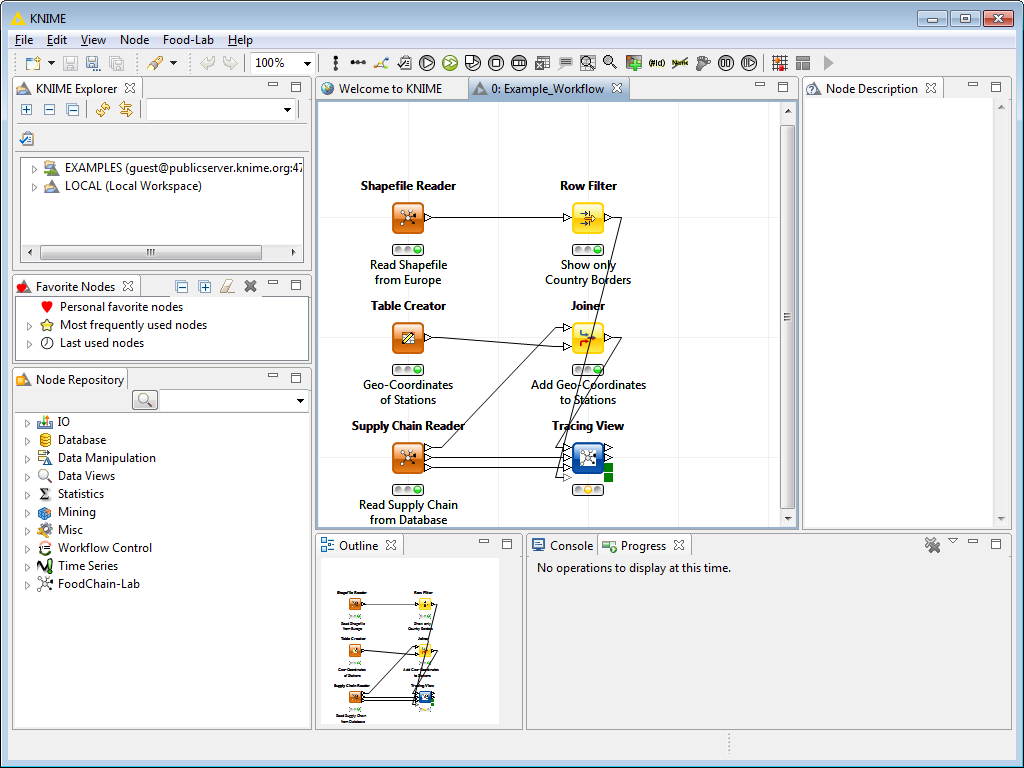
\includegraphics[height=0.6\textheight]{1.png}
	\end{center}
	\begin{itemize}
		\item x
	\end{itemize}
\end{frame}

\end{document}
